\documentclass{article}
\usepackage{settings}
\date{\today}
\begin{document}
\thispagestyle{empty}
\begin{center}
    \LARGE\textbf{МИНОБРНАУКИ РОССИИ\\
        САНКТ-ПЕТЕРБУРГСКИЙ ГОСУДАРСТВЕННЫЙ\\
        ЭЛЕКТРОТЕХНИЧЕСКИЙ УНИВЕРСИТЕТ\\
        "ЛЭТИ"\ ИМ. В.И.УЛЬЯНОВА(ЛЕНИНА)\\
        Кафедра МО ЭВМ}\\[4cm]
    \Large\textbf{ОТЧЁТ}\\[0.2cm]
    \Large\textbf{по учебной практике}\\[0.1cm]
    \Large\textbf{по дисциплине <<Генетические алгоритмы>>}\\[0.1cm]
    \Large\textbf{Тема: Алгоритм Рюкзака.}\\[2cm]
\end{center}
\Large{Студент гр. 1304 \qquad \qquad \quad \underline{\hspace{6cm}} \qquad \qquad Мусаев А.И.}\\[0.25cm]
\Large{Студент гр. 1304 \qquad \qquad \quad \underline{\hspace{6cm}} \qquad \qquad Поршнев Р.А.}\\[0.25cm]
\Large{Студентка гр. 1381 \qquad \quad \quad \underline{\hspace{6cm}} \qquad \qquad Демчук П.Д.}\\[0.25cm]
\Large{Преподаватель \qquad \qquad \qquad \underline{\hspace{6cm}} \qquad \qquad Жангиров Т.Р.}\\[1cm]
\begin{center}
    Санкт-Петербург\\
    2023
\end{center}
\newpage

\textbf{Задание}

Пусть имеется набор предметов, каждый из которых имеет два параметра — масса и ценность. Также имеется рюкзак определённой грузоподъёмности. Задача заключается в том, чтобы собрать рюкзак с максимальной (или близкой к максимальной) ценностью предметов внутри, соблюдая при этом ограничение рюкзака на суммарную массу.

\textbf{Выполнение работы}

\textbf{03.07 - 1 итерация}

\begin{enumerate}
\item GUI был спроектирован в Qt Designer. 

\begin{figure}[h!]
\centering
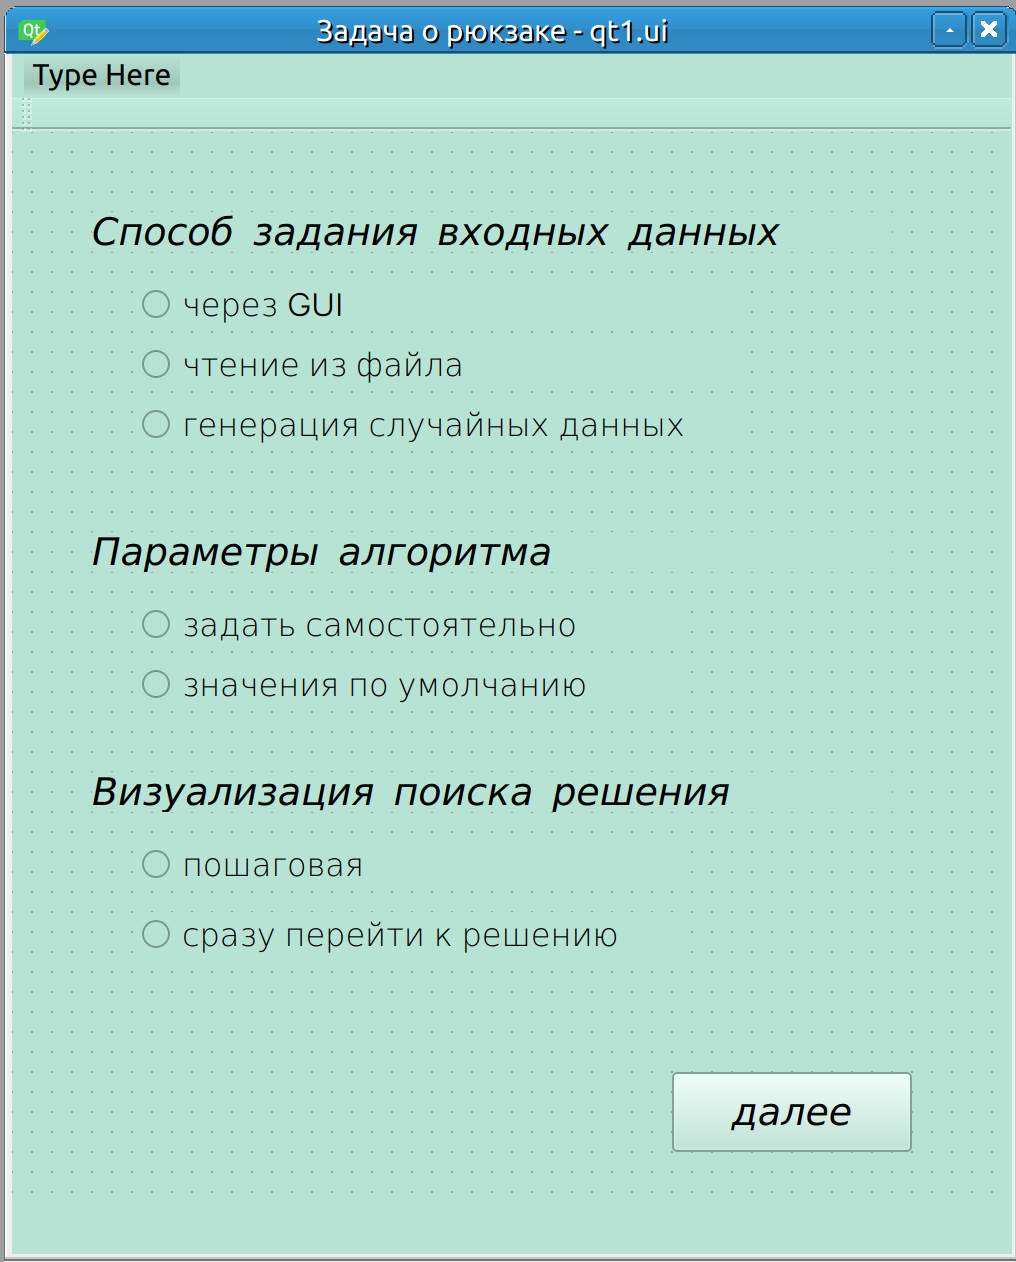
\includegraphics[width=0.5\linewidth]{images/qt1.png}
\caption{Начальная настройка работы с алгоритмом}
\label{fig:mpr}
\end{figure}

\begin{figure}[h!]
\begin{minipage}[h]{0.32\linewidth}
\center{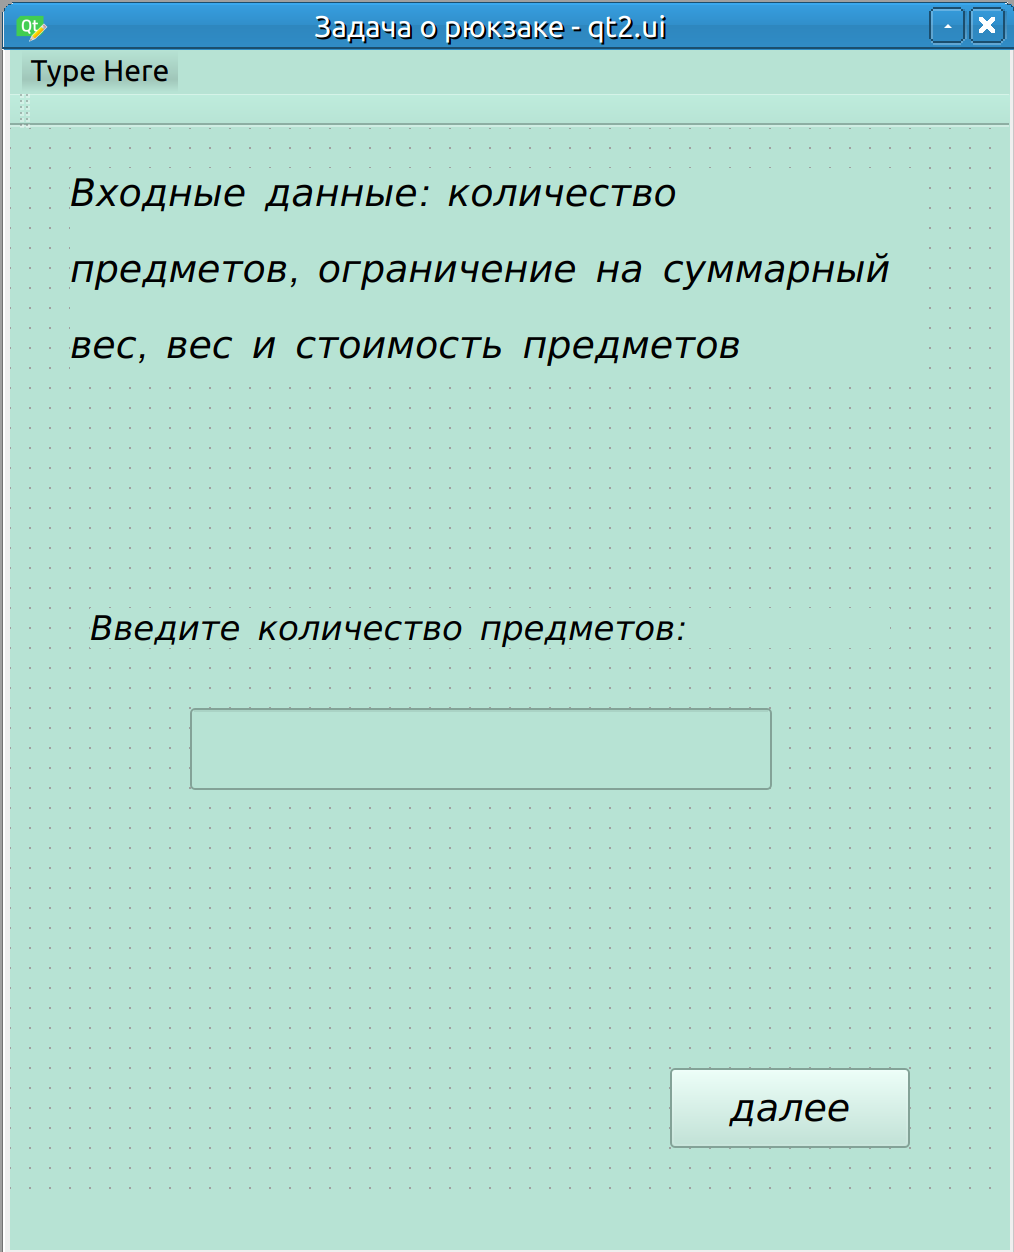
\includegraphics[width=1\linewidth]{images/qt2.png}}
\end{minipage}
\hfill
\begin{minipage}[h]{0.32\linewidth}
\center{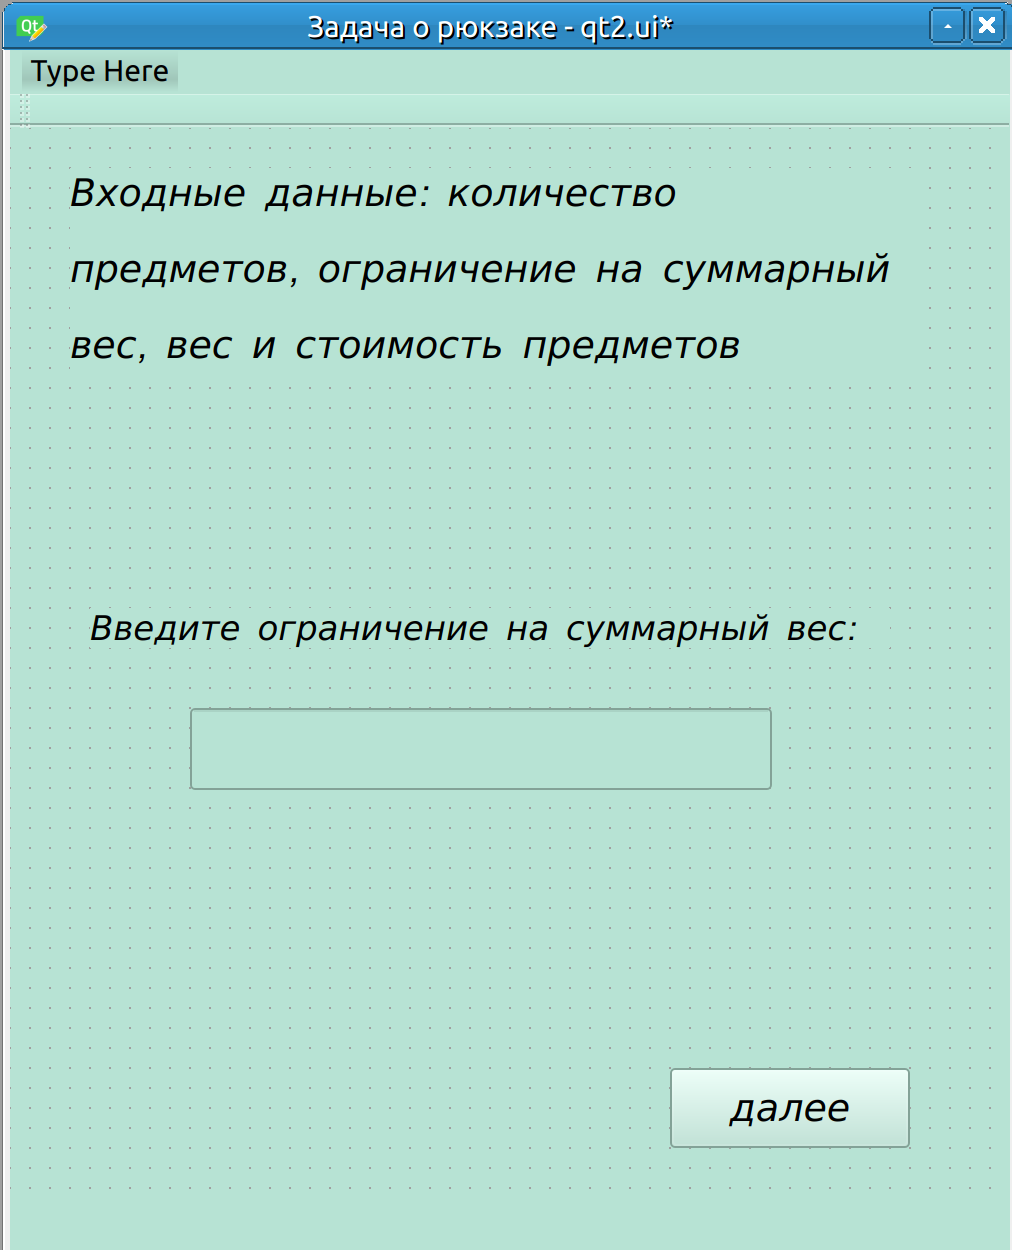
\includegraphics[width=1\linewidth]{images/qt2_2.png}}
\end{minipage}
\hfill
\begin{minipage}[h]{0.32\linewidth}
\center{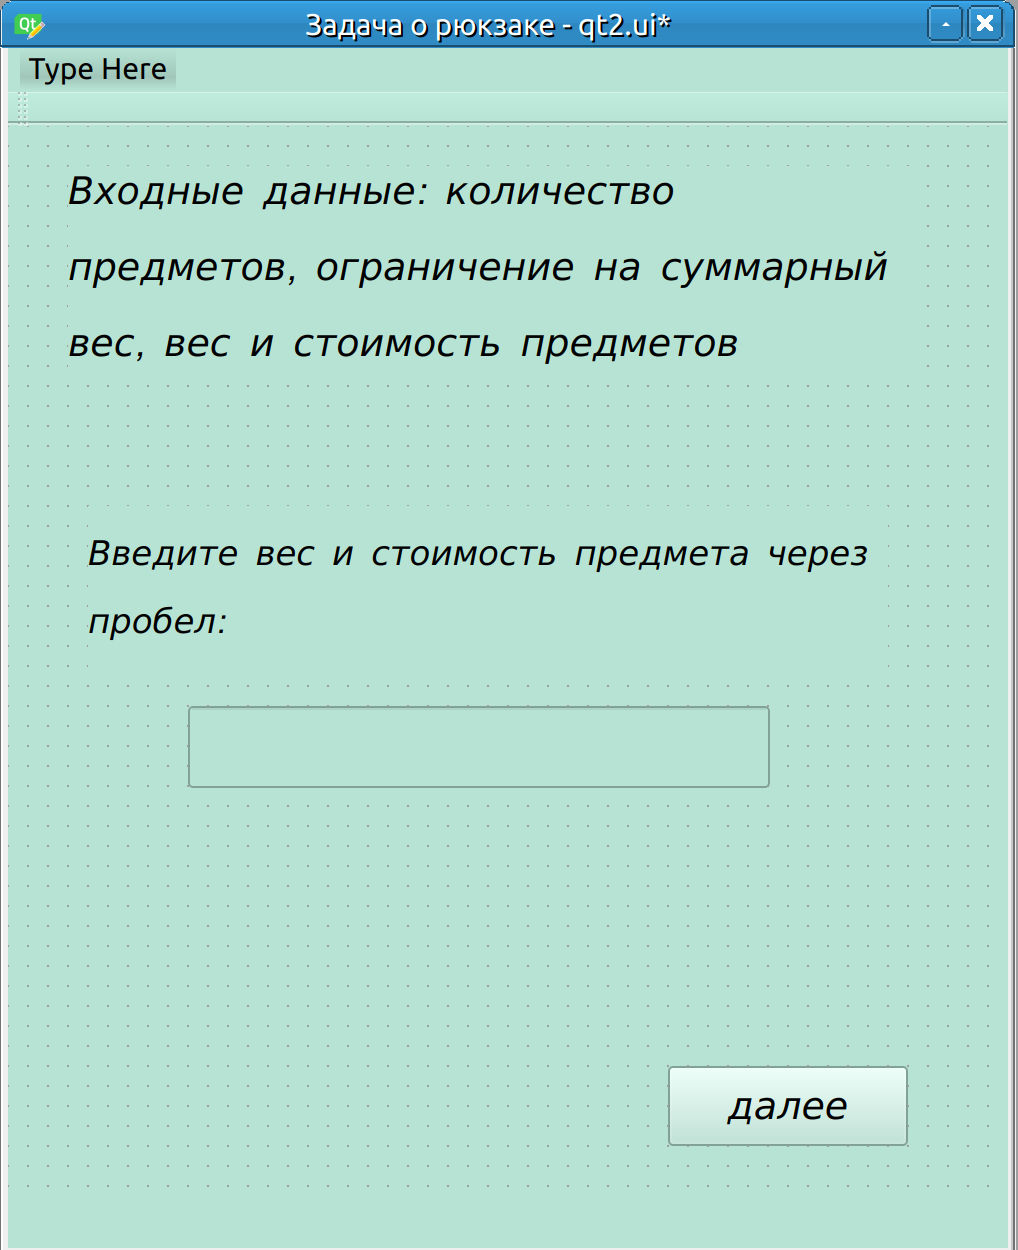
\includegraphics[width=1\linewidth]{images/qt2_3.png}}
\end{minipage}
\caption{Считывание входных данных}
\label{ris:image1}
\end{figure}

\begin{figure}[h!]
\begin{minipage}[h]{0.32\linewidth}
\center{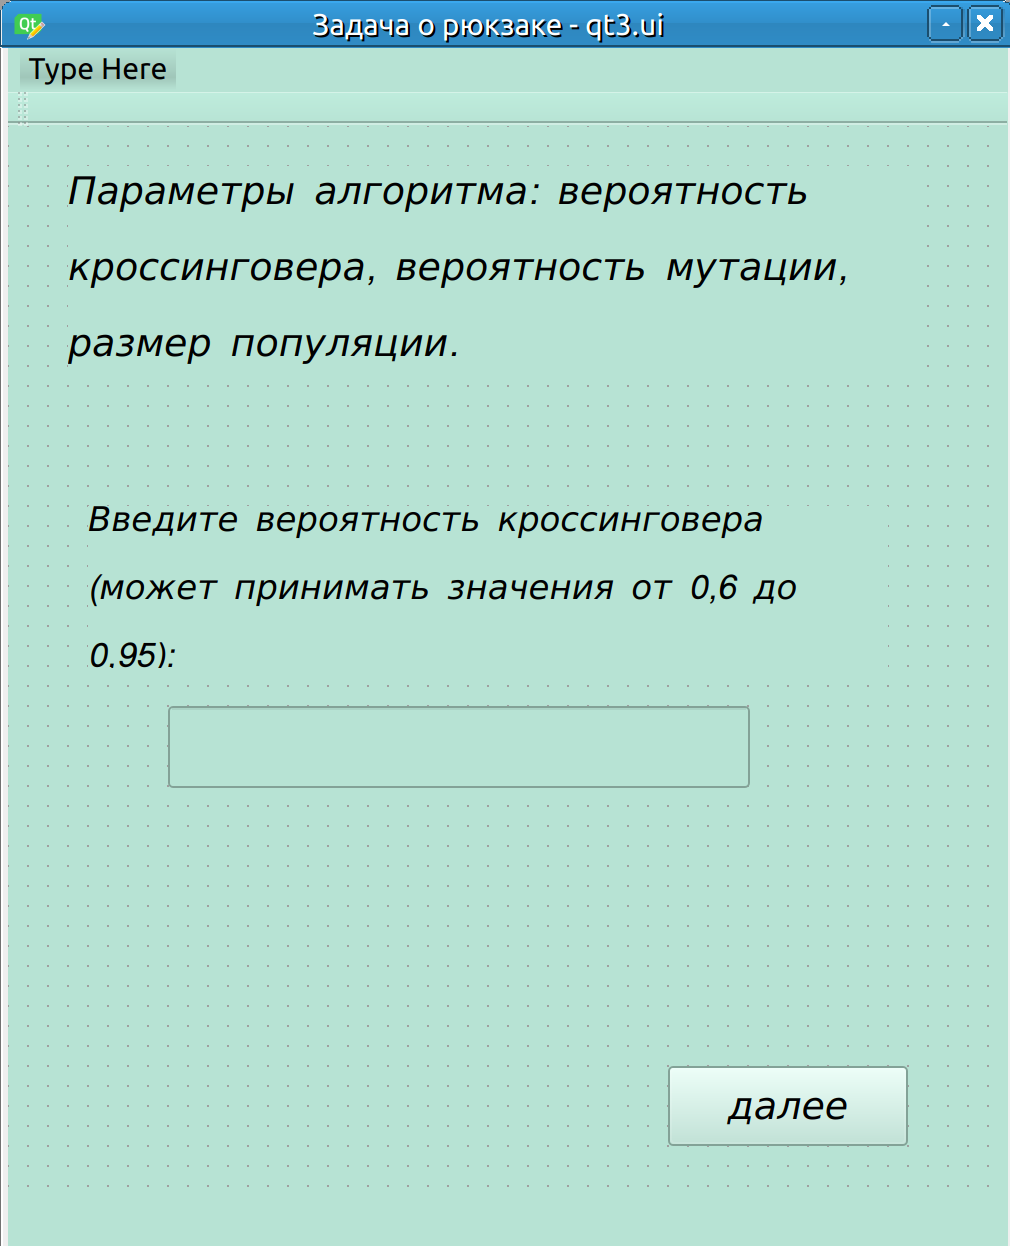
\includegraphics[width=1\linewidth]{images/qt3.png}}
\end{minipage}
\hfill
\begin{minipage}[h]{0.32\linewidth}
\center{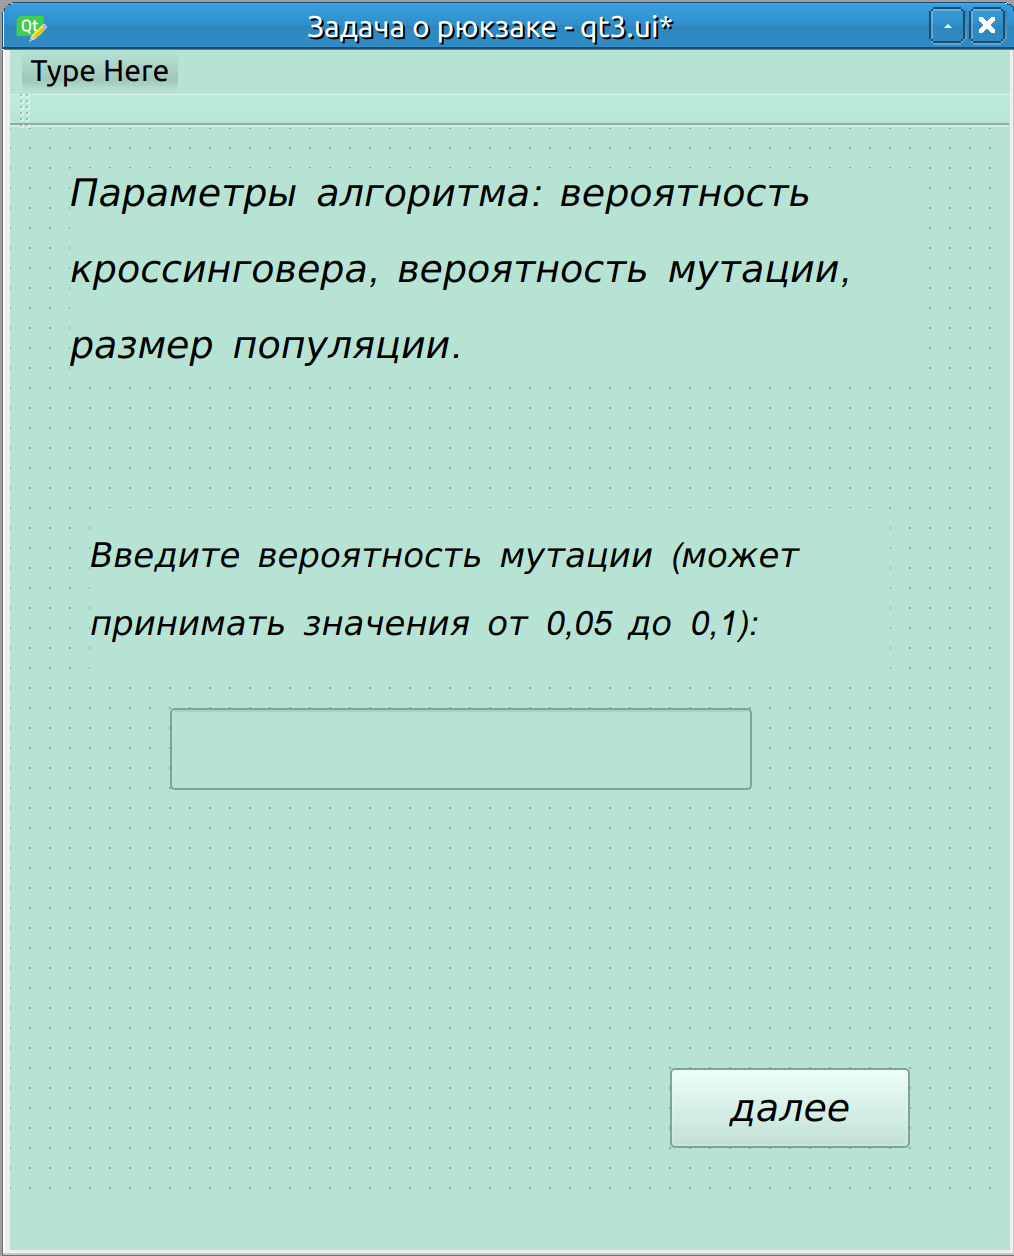
\includegraphics[width=1\linewidth]{images/qt3_2.png}}
\end{minipage}
\hfill
\begin{minipage}[h]{0.32\linewidth}
\center{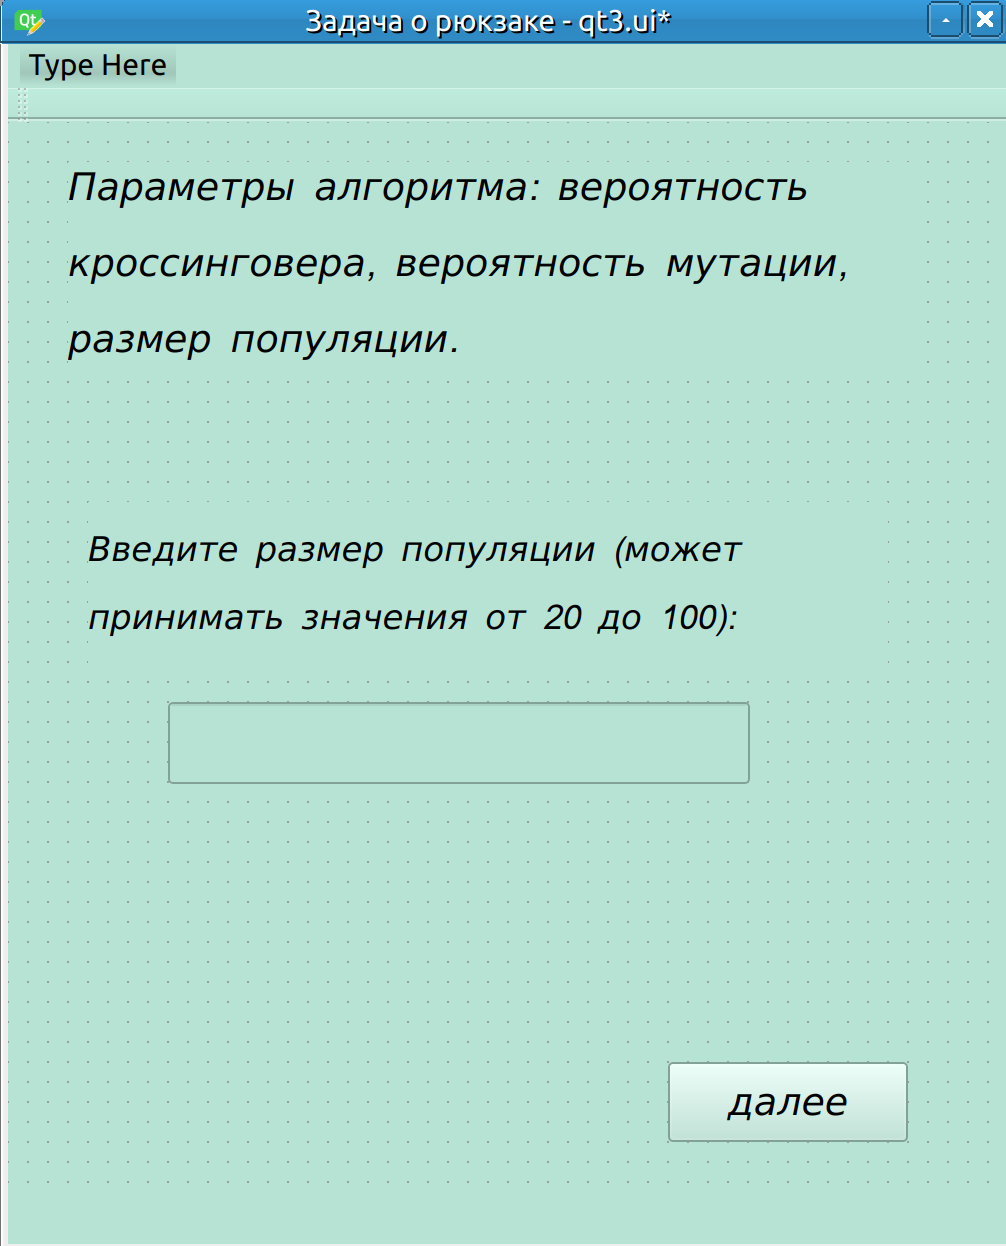
\includegraphics[width=1\linewidth]{images/qt3_3.png}}
\end{minipage}
\caption{Задание значений для работы алгоритма}
\label{ris:image1}
\end{figure}

\newpage

\item Модификации генетического алгоритма

Выбор родителей будет происходить турнирным отбором, так метод рулетки с большей вероятностью сведётся к жадному алгоритму, что невыгодно для решения задачи о рюкзаке.

Формирование пар родителей будет производиться сначала по принципу аутбридинга, а в конце работы алгоритма глобальные экстремумы будут уточняться по принципу инбридинга. 

Рекомбинация пар будет происходить при помощи однородного кроссинговера, так как данный способ гарантирует, что в строке-потомке будут чередоваться короткие строки особей-родителей. 

Мутация для каждой полученной особи будет происходить самоадаптирующимся способом при помощи критерия расстояния, то есть вероятность мутации каждого гена потомка будет равна: 

{
\Large
\begin{center}
$P_r(A,B) = M(A,B)M_m = (1 - dist(A,B))M_m$, где

$dist(A,B) = \frac{1}{n}\sum_{i=1}^n\frac{a_i-b_i}{max_i-min_i}^d$, $d=0,2$ и $M_m=0,9$
\end{center}
}

Для отбора популяции будет использоваться отбор вытеснением, так как данный способ даёт возможность собрать наиболее разнообразный рюкзак, то есть находить несколько глобальных экстремумов, а также данный способ является наиболее надёжным.

В дальнейшем будет добавлена возможность выбора методов, на основе которых выполняется генетический алгоритм.

\item Метрики генетического алгоритма

Пользователю будет предоставлена возможность задавать метрики самостоятельно либо по умолчанию. В случае задания вероятности кроссинговера самостоятельно её значения должно варьироваться в пределе от 0.6 до 0.95, для мутации - от 0.005 до 0.01 (в случае выбора самоадаптирующейся мутации данный функционал пользователю недоступен), а размер популяции - от 20 до 100 особей. По умолчанию будут использованы следующие метрики: вероятность мутации равна 0.01 (не применимо для самоадаптирующейся мутации), вероятность кроссинговера равна 0.8, размер популяции равен 30 особям.

\item Описание структур данных для хранения

Чтобы хранить поданные в генетический алгоритм данные будет использоваться массив кортежей, в котором каждому предмету будет соответствовать кортеж (цена, вес).

Для хранения отдельной хромосомы будет использован тип str, который будет хранить двоичное число (1 - предмет взять в данном наборе, 0 - отсутствует). Популяция же будет состоять из списка строк. Также будет использоваться список, каждый элемент которого будет хранить кортеж вида - (суммарная стоимость генотипа, суммарный вес генотипа). Оба вышеоуказанных массива будут храниться в структуре, которая характеризует популяцию. 

\item Стек технологий

Для реализации GUI будет использоваться библиотека PyQt, а для отрисовки графиков функции качества -- Matplotlib.

\item Распределение ролей в бригаде

Студент Мусаев Артур ответственный за проектировку и хранение данных, студентка Демчук Полина ответственная за разработку GUI, студент Поршнев Роман ответственный за разработку архитектуры.

\end{enumerate}

\newpage

\textbf{Заключение}

\textbf{01.07}

На данной итерации были частично распределены роли, выбраны модификации и метрики работы алгоритма. Разработана макет GUI. Кроме того, была создана архитектура проекта.

\textbf{06.07 - 2 итерация}

\begin{enumerate}
\item Исправление замечаний в GUI

На странице ввода предметов была добавлена кнопка для удаления последнего введенного предмета.

На странице задания значений параметров для работы алгоритма строка для ввода была заменена на spinbox для того, чтобы избежать обработку неверно введенных данных, так как параметры могут принимать ограниченное количество значений.

В прототипе страницы визуализации работы алгоритма формат представления рекорда был заменен на табличный вид (столбцы - номера предметов, строки - их вес и стоимость). Также добавлена кнопка замены параметров алгоритма для его перезапуска.

\item Реализация GUI

Вспомогательные классы: \textit{Page1RadioButtons} -  данный класс имеет только конструктор, который размещает виджеты на главном окне (для страницы 1 - выборы опций). \textit{Page2InputData} - имеет конструктор и метод \textit{page2\_mod}, который отрисовавает модификацию страницы 2 (ввод входных данных) и считывает данные введеные пользователем. \textit{Page3ParamsOfAlg} - имеет конструктор и метод \textit{page3\_mod}, который отрисовавает модификацию страницы 3 (ввод параметров алгоритма). \textit{Page4Vizualization} - отрисовка 4 страницы (пошаговое отображение работы алгоритма).

Главный класс \textit{Window} - класс, объект которого - главное окно. Реализует логику GUI и инициализирует само окно. В конструкторе задаются такие параметры окна, как размер, цвет, название, инициализируются поля, значения которых будут переданы в алгоритм, и вызывается конструктор класса \textit{Page1RadioButtons}. Класс имеет следующие методы:

\textit{group1Response(btn), group2Response(btn)} - методы для разных групп радио кнопок (1 группа - способ задания входных данных, 2 группа - параметры алгоритма. Они вызываются при нажатии на радио кнопку, и записывают строкой в поле класса \textit{group1res (group2res)}, какая кнопка была нажата. 

\textit{chooseTypeOfInput} - метод вызывается при попытке пользователем нажать кнопку "далее" на первой странице. Происходит проверка, в каждой ли группе радио кнопок совершен выбор. Если нет, генерируется сообщение об ошибке, если да, то на основании выбранных опций вызывается метод/конструктор другого класса для отрисовки следующей страницы.

\textit{page2\_mod} - вызывает отрисовку второй модификации окна 2 после ввода ограничения на суммарный вес и нажатия enter.

\textit{choseTypeOfParam} - проверяет какая кнопка была нажата в группе 2 и либо вызывает конструктор класса \textit{Page3ParamsOfAlg} (отрисовка 3 страницы), либо переходит к проверке следующей группы радио кнопок.

\textit{errorMes(mes: str)} - генерирует всплывающее окно с сообщением об ошибке. Аргумент - сообщение.

\textit{page2withFileInput} - вызывается если пользователь выбрал ввод входных данных через загрузку файла. Создает объект класса \textit{SecondWindow} - новое окно, через которое будет произведена загрузка файла. Внутри конструктора класса SecondWindow создается виджет - объект класса \textit{FileLabel}, обладающий функционалом drag\&drop. При нажатии кнопки "далее", проверяется корректный ли файл загружен. Если да, то путь к этому файлу отправляется в родительское (главное) окно и окно2 закрывается. Если нет, то генерируется всплывающее сообщение об ошибке.

\textit{getFilePath(url: str)} - записывает путь к файлу, полученный из дочернего окна, в поле класса pathToFile.

\textit{page2\_mod} - вызывает отрисовку второй модификации окна 3 после ввода первого параметра и нажатия кнопки "далее".

\textit{choseTypeOfVisual} - определяет следующую страницу для отрисовки по выбору опции в группе 3 радио кнопок.

\textit{preparingDataForAlg} - метод, создающий объект класса \textit{DataPacking}, который запаковывает все данные, введенные пользователем, в структуру для последующей передачи в алгоритм.

\textit{Класс DataPacking} - заполняет структуру данных в зависимости от опций выбранных пользователем (в конструкторе). При неоходимости генерации случайных данных вызывается метод \textit{data\_generator}.

\item Генетический алгоритм был частично реализован и выполняет поставленную задачу:

\begin{figure}[h]

\centering

\includegraphics[width=0.8\linewidth]{images/test1.jpeg}

\caption{Сравнение с динамическим алгоритмом}

\label{fig:mpr}

\end{figure}

Для мутации пока что была реализована только мутация с заменой 0 на 1 и наоборот, вероятность может задать либо пользователь, либо по умолчанию она задается критерием расстояния.

Для выбора пар родителей были реализованы: панмиксия, аутбридинг и инбридинг

Для выбора родителей был реализован турнирный отбор.

Для выбора популяции были реализованы отбор вытеснением и элитарный отборы.

Генетический алгоритм оперирует такими структурами данных как списки, а именно: список популяции, список отобранных родителей, список список пар родителей и список потомков. На начальном этапе список популяции получается с помощью случайной генерации, затем отбираются родители, далее пары родителей, потомки и последний шаг итерации -- это отбор особей в новую популяцию.
\end{enumerate}

\textbf{Заключение}

Была реализована большая часть GUI и частично реализован ГА.

\textbf{10.07 - 3 итерация}

\begin{enumerate}
\item Реализация GUI

Добавлен класс \textit{Page4Vizualization}, конструктор которого отрисовывает страницу визуализации решения. Метод \textit{changeRowColor (chromosome: str)} перекрашивает ячейки в таблице, если предмет взят для данной хромосомы.

Класс \textit{Window} дополнен следующими методами:

\textit{ShowStep(step: int)} - отображает соответсвующий шаг алгоритма.

\textit{PrevStepOfAlg} - вызывает отображение предыдущего шага алгоритма, если он существует, в ином случае - генерирует сообщение об ошибке.

\textit{NextStepOfAlg} - вызывает отображение следующего шага алгоритма, если он существует, в ином случае - генерирует сообщение об ошибке.

\textit{ShowLastStepOfAlf} - вызывает отображение последнего шага алгоритма.

\textit{RestartAlgWithNewParams} - вызывает конструктор класса \textit{Page3ParamsOfAlg}, который отрисовывает окно с выборами параметров алгоритма, для ввода новых опций и перезапуска алгоритма.

\item Доработка алгоритма

Генетический алгоритм был полностью реализован. В зависимости от модификаций можно использовать разные модули ген. алгоритма. 

Кроме того, был добавлен критерий останова. он работает так: если на последних 1000 итераций ответ не меняется, выводится найденный.

Имеются следующие модификации:

Варианты выбора родителей: Турнирный отбор, Рулетка.

Варианты составления пар: Панмиксия, Инбридинг + Аутбридинг.

Варианты кроссоверов: Однородная, Одноточечная.

Варианты выбора популяции: Элитарный, Вытеснением.

Варианты мутаторов: Двоичный, Адаптивный.

\item Тестирование и визуализация

Тест 1

Входные данные:

Веса предметов: 238, 405, 135, 177, 610, 197, 276, 522, 250, 398.

Стоимости предметов: 38, 63, 39, 32, 7, 15, 37, 41, 93, 46.

Вместительность рюкзака: 394.

Вероятность кроссинговера: 0.8.

Размер популяции: 20.

Модификации: турнирый отбор родителей, сочетание аутбридинга и инбридинга, однородный кроссинговер, самоадаптирущийся мутатор, элитарный отбор популяции.

Выходные данные представлены на Рисунке 5.
\begin{figure}[h!]
\centering
\includegraphics[width=1.0\linewidth]{images/test1.png}
\caption{Результаты работы алгоритма}
\label{fig:mpr}
\end{figure}

Тест 2

Входные данные:

Веса предметов: 285, 290, 6, 40, 238, 228, 408, 215, 235, 434, 559, 44, 534, 213.

Стоимости предметов: 23, 55, 63, 100, 22, 38, 68, 84, 68, 25, 30, 94, 82, 65.

Вместительность рюкзака: 341.

Вероятность кроссинговера: 0.85.

Вероятность мутации: 0.0005.
Размер популяции: 25.

Модификации: турнирый отбор родителей, сочетание аутбридинга и инбридинга, однородный кроссинговер, двоичный мутатор, элитарный отбор популяции.

Выходные данные представлены на Рисунке 6.
\begin{figure}[h!]
\centering
\includegraphics[width=1.0\linewidth]{images/test2.png}
\caption{Результаты работы алгоритма}
\label{fig:mpr}
\end{figure}

Тест 3

Входные данные:

Веса предметов: 46, 525, 476, 381, 26, 269, 312, 604, 653, 123, 648, 629, 347, 181, 540, 460.

Стоимости предметов: 12, 43, 70, 66, 98, 88, 42, 73, 3, 37, 36, 53, 7, 76, 17, 35.

Вместительность рюкзака: 112.

Вероятность кроссинговера: 0.7.

Размер популяции: 30.

Модификации: турнирый отбор родителей, сочетание аутбридинга и инбридинга, одноточечный кроссинговер, самоадаптирующийся мутатор, элитарный отбор популяции.

Выходные данные представлены на Рисунке 7.
\begin{figure}[h!]
\centering
\includegraphics[width=1.0\linewidth]{images/test3.png}
\caption{Результаты работы алгоритма}
\label{fig:mpr}
\end{figure}

Тест 4

Входные данные:

Веса предметов: 671, 385, 301, 6, 208, 96, 490, 369, 222, 193, 286, 669, 485, 118, 135, 4, 333, 211, 431, 31.

Стоимости предметов: 84, 70, 18, 24, 32, 97, 16, 36, 12, 45, 14, 74, 36, 15, 96, 88, 34, 1, 32, 84.

Вместительность рюкзака: 203.

Вероятность кроссинговера: 0.7.

Вероятность мутации: 0.01.

Размер популяции: 30.

Модификации: турнирый отбор родителей, панмиксия, однородный кроссинговер, двоичный мутатор, элитарный отбор популяции.

Выходные данные представлены на Рисунке 8.
\begin{figure}[h!]
\centering
\includegraphics[width=1.0\linewidth]{images/test4.png}
\caption{Результаты работы алгоритма}
\label{fig:mpr}
\end{figure}

Тест 5

Входные данные:

Веса предметов: 97, 474, 178, 236, 33, 377, 274, 12, 436, 614, 79, 202, 571, 454, 387, 54, 406, 487, 401, 293, 376, 25, 468, 676, 615, 118, 352, 323, 45, 271, 310, 2, 138, 580, 128, 444, 529, 93, 597, 279, 491, 508, 218, 175, 348, 67, 202, 642, 480, 646, 479, 510, 420, 586, 479, 99, 317, 522, 86, 441, 295, 33, 252, 682, 698, 645, 195, 543, 259, 551, 32, 74, 195, 59, 532, 10, 471, 461, 525, 308, 477, 605, 543, 664, 197, 105, 502, 569, 70, 137, 190, 195, 628, 36, 497, 92, 155, 212, 643, 602.

Стоимости предметов: 95, 65, 55, 46, 97, 9, 41, 20, 66, 98, 54, 38, 99, 37, 73, 47, 19, 48, 4, 17, 7, 54, 83, 71, 38, 33, 68, 57, 24, 27, 69, 35, 93, 95, 60, 4, 26, 43, 47, 93, 6, 62, 83, 15, 52, 70, 49, 90, 32, 26, 47, 27, 10, 30, 21, 87, 39, 89, 73, 49, 96, 81, 73, 57, 34, 14, 84, 21, 25, 11, 3, 98, 40, 27, 39, 52, 97, 33, 75, 25, 45, 91, 99, 2, 8, 50, 80, 13, 69, 55, 19, 84, 68, 26, 19, 94, 39, 76, 23, 87.

Вместительность рюкзака: 247.

Вероятность кроссинговера: 0.95.

Вероятность мутации: 0.0095.

Размер популяции: 40.

Модификации: рулеточный отбор родителей, панмиксия, одноточечный кроссинговер, самоадаптирующийся мутатор, элитарный отбор популяции.

Выходные данные представлены на Рисунке 9.
\begin{figure}[h!]
\centering
\includegraphics[width=1.0\linewidth]{images/test5.png}
\caption{Результаты работы алгоритма}
\label{fig:mpr}
\end{figure}

\newpage

\textbf{Заключение}

Разработано приложение c GUI на языке Python3, решающее задачу о рюкзаке с помощью генетического алгоритма. Реализовано несколько модификаций генетического алгоритма, а также реализован ввод параметров генетического алгоритма. Данный алгоритм приближённо решает поставленную задачу.
\end{enumerate}

\end{document}

